\documentclass[tikz,border=3mm,multi=tikzpicture]{standalone}
\usepackage{tikz}
\usetikzlibrary{arrows.meta,positioning}
\begin{document}
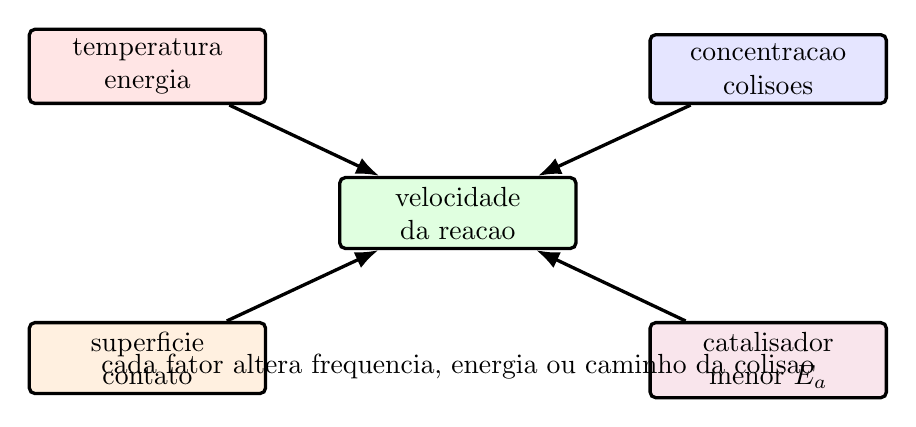
\begin{tikzpicture}[>=Latex,node distance=0.65cm]
  \tikzstyle{box}=[draw,rounded corners=2pt,very thick,minimum width=3cm,minimum height=0.8cm,align=center]
  \node[box,fill=green!12] (vel) {velocidade\\da reacao};
  \node[box,fill=red!10,above left=0.9cm and 0.9cm of vel] (temp) {temperatura\\energia};
  \node[box,fill=blue!10,above right=0.9cm and 0.9cm of vel] (conc) {concentracao\\colisoes};
  \node[box,fill=orange!12,below left=0.9cm and 0.9cm of vel] (surf) {superficie\\contato};
  \node[box,fill=purple!10,below right=0.9cm and 0.9cm of vel] (cat) {catalisador\\menor $E_a$};
  \draw[very thick,->] (temp) -- (vel);
  \draw[very thick,->] (conc) -- (vel);
  \draw[very thick,->] (surf) -- (vel);
  \draw[very thick,->] (cat) -- (vel);
  \node[align=center,below=1.2cm of vel] {cada fator altera frequencia, energia ou caminho da colisao};
\end{tikzpicture}

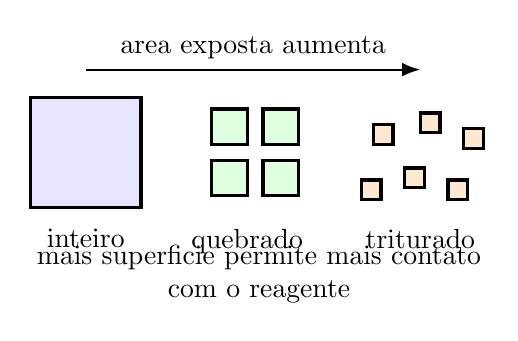
\begin{tikzpicture}[x=1cm,y=1cm,>=Latex]
  \draw[fill=blue!10,very thick] (0,0) rectangle (1.4,1.4);
  \node[below] at (0.7,-0.15) {inteiro};
  \foreach \x/\y in {2.3/0.15,2.95/0.15,2.3/0.8,2.95/0.8}{
    \draw[fill=green!12,very thick] (\x,\y) rectangle +(0.45,0.45);
  }
  \node[below] at (2.75,-0.15) {quebrado};
  \foreach \x/\y in {4.2/0.1,4.75/0.25,5.3/0.1,4.35/0.8,4.95/0.95,5.5/0.75}{
    \draw[fill=orange!18,very thick] (\x,\y) rectangle +(0.25,0.25);
  }
  \node[below] at (4.95,-0.15) {triturado};
  \draw[->,thick] (0.7,1.75) -- node[above] {area exposta aumenta} (4.95,1.75);
  \node[align=center] at (2.9,-0.85) {mais superficie permite mais contato\\com o reagente};
\end{tikzpicture}
\end{document}
